
\section{Whitted Rendering}
In his 1980 paper\cite{whitted_improved_1980}, J. Turner Whitted
introduced the notion of recursive raytracing.

\subsection{The illumination model}
The light from an object to the viewer consist of a specular reflection \(S\),
a transmission reflection \(T\) and a diffusive component \(D\).
Thus the Whitted model is given by the equation

\begin{equation}
    \label{eq:whitted_model}
    I = I_a + \sum_j D(\vec L_j) + k_sS + k_t T,
\end{equation}


where
\begin{itemize}
    \item \(I\) is the reflected intensity,
    \item \(I_a\) is the reflection due to ambient lighting,
    \item \(k_t\) the transmission coefficient,
    \item \(k_s\) is the specular reflection constant,
    \item \(\vv{N}\) is the unit surface normal,
    \item \(\vv R\) is the reflected direction,
    \item \(\vv P\) is the refracted direction,
    \item \(\vv*{L}{j}\) is the vector in the direction of the \(j\)th light source,
    \item \(S\) is the intensity of light incident from the direction \(\vv R\),
    \item \(T\) is the intensity of light incident from the direction \(\vv P\),
    \item Finally, \(D(\vv a)\) gives the diffuse contribution comming from direction \(\vv a\)
\end{itemize}

Note that both \(\vv{R}\) and \(\vv{P}\) are computed thanks to the Snell-Descartes formulas.

\begin{center}
    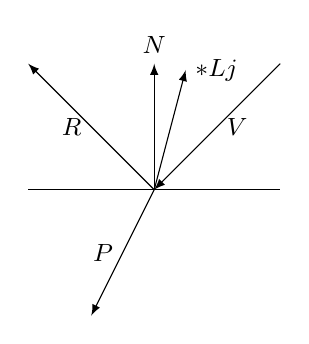
\begin{tikzpicture}[scale=0.8, font=\small]
        \draw         (-2,0) -- (2,0);
        \draw [-latex] (0,0) -- (0,2)  node [above] {\(\vv{N}\)};
        \draw [-latex] (2,2) -- (0,0) node [midway,  right] {\(\vv{V}\)};
        \draw [-latex] (0,0) -- (-2,2) node [midway, left] {\(\vv{R}\)};
        \draw [-latex] (0,0) -- (-1,-2) node [midway, left] {\(\vv{P}\)};
        \draw [-latex] (0,0) -- (0.5,1.9) node [right] {\(\vv*{L}{j}\)};
    \end{tikzpicture}

    \captionof{figure}{The vectors useful in the Whitted illumination model}
\end{center}


To compute \(S\) and \(T\), one need to cast rays more rays until a maximum depth has been reached when the ray does not intersect any object.

\subsection{Variations and subtilities}
The function \(D\) should check whether path between the object and the light is not obstructed. If so, the light cannot contribute to the illumination.
To check whether the contribution of a light should be taken into consideration, a \textit{shadow ray} is cast from the light up to the surface to check intersection with objects.

Due to how the whitted illumination works, emissive materials can't work out of the box because emissive lightning require diffuse rays to be cast, grabing light from all incoming direction  and not only from light.
A way to circumvent this limitation would be to detect emissive materials and consider them as area light in the diffuse calculation.